\documentclass[11pt,a4paper]{article}

\usepackage[margin=2.5cm]{geometry}
\usepackage{amsmath,amssymb,amsthm}
\usepackage{stmaryrd}
\usepackage{hyperref}
\usepackage{enumitem}
\usepackage{booktabs}
\usepackage{tikz}
\usetikzlibrary{arrows.meta,positioning,chains,trees}
\usepackage{tikz-cd}

\hypersetup{
  colorlinks=true,
  linkcolor=blue!70!black,
  citecolor=green!50!black,
  urlcolor=blue!60!black
}

\newcommand{\Set}{\mathbf{Set}}
\newcommand{\Poly}{\mathbf{Poly}}
\newcommand{\cont}[2]{#1 \triangleleft #2}
\newcommand{\Ext}[1]{\llbracket #1 \rrbracket}
\newcommand{\N}{\mathcal{N}}
\newcommand{\B}{\mathcal{B}}
\newcommand{\dc}{\mathbin{\downarrow}}
\newcommand{\obs}{\mathsf{o}}
\newcommand{\site}{\mathrm{site}}
\newcommand{\Fac}{\mathrm{Fac}}
\newcommand{\Prod}{\mathrm{Prod}}

\theoremstyle{plain}
\newtheorem{theorem}{Theorem}[section]
\newtheorem{proposition}[theorem]{Proposition}

\theoremstyle{definition}
\newtheorem{definition}[theorem]{Definition}
\newtheorem{example}[theorem]{Example}
\newtheorem{construction}[theorem]{Construction}

\theoremstyle{remark}
\newtheorem{remark}[theorem]{Remark}
\newtheorem{slogan}[theorem]{Slogan}

\title{\textbf{Supply Chains as Directed Containers}}

\author{Robin Langer \and Claude}

\date{July 2026}

\begin{document}
\maketitle

\begin{abstract}
We describe supply chains using the language of containers and directed
containers, climbing a ladder of examples while the formalism stands
still. The shipping network of \emph{Sawasdee Cellars}, an Australian
wine exporter selling into Thailand, is a finite tree, and its free
category is a directed container (and therefore a comonad);
cold-chain integrity, tariffs, markups, and licensing compliance are
monoid-valued tracking functors on it. \emph{Falcon Steel}, a
producer in the United
Arab Emirates, adds a second tree---the bill of materials---as a
second directed container, with sourcing a functor connecting it to
the network. Alternative routings then make the network a DAG, and
recycling closes a cycle, making it a graph in earnest; at every rung
the constructions apply unchanged. Aggregation and demand fulfilment
are cofunctors, and inventory dynamics form an update monad. The
distinction between the flow of goods (functors) and the flow of
demand (cofunctors) is genuine and irreducible; following
Fairbanks--Carlson--Spivak, the two coexist in a double category. This
is an expository note---no new theorems, just a translation exercise to
build intuition. All constructions are mechanically verified in
Lean~4.
\end{abstract}

%% ============================================================
\section{Introduction}

Supply chain management is a discipline of local records that must
cohere globally: temperatures logged per leg but certified per
journey, margins taken per hand-off but audited in the shelf price,
parts lists written per product but costed per finished good. The
mathematics of local views that cohere is the theory of comonads,
and the comonads relevant here have a concrete combinatorial form:
\emph{directed containers}, equivalently small categories,
equivalently comonoids in $\Poly$. This note translates the standard
vocabulary of supply chains into that language, one term at a time.

The note is organized as a ladder of examples on which the
formalism never changes---only the underlying graph does.
Section~\ref{sec:setup} fixes the running example, Sawasdee
Cellars, a Melbourne agency exporting South Australian shiraz to
Thailand; Section~\ref{sec:glossary} is a glossary of supply-chain
terms, aimed at a reader who knows what a comonad is but not what a
duty point is; Section~\ref{sec:dcont} recalls containers and
directed containers. Then the ladder. \emph{Trees}: the wine
network is a tree, and cold chain, tariffs, markups, and licensing
are monoid-valued tracking functors on its free category
(Section~\ref{sec:network}); Falcon Steel, a producer in the United
Arab Emirates, adds a second tree, the bill of materials, with
sourcing a functor connecting the two (Section~\ref{sec:steel}).
\emph{DAGs}: alternative routings give the network several routes
between the same endpoints, and repeated components do the same for
the BOM (Section~\ref{sec:dag}). \emph{Graphs}: the mill's scrap
loop closes a cycle, and the free category takes it in stride
(Section~\ref{sec:graph}). With the flow of goods in place,
Section~\ref{sec:cofunctors} turns to the flow of demand:
aggregation and fulfilment are cofunctors, which coexist with
functors in a double category but merge with them in neither
direction. Section~\ref{sec:inventory} models inventory as an
update monad. Section~\ref{sec:formalization} records the Lean~4
formalization of every construction in the note, and
Section~\ref{sec:outlook} points at dynamics.

%% ============================================================
\section{Setup: Simplified Supply Chain}\label{sec:setup}

We work with a stripped-down model. A supply chain has:

\begin{itemize}[nosep]
\item A set $\Fac$ of \textbf{facilities}: vineyards, export
  agencies, ports, distributors, retailers.
\item A set of \textbf{shipping legs}: a leg $f \to g$ means goods can
  move directly from facility $f$ to facility $g$. Facilities and legs
  form a directed graph $G$.
\item \textbf{Per-leg tracking data}: each shipping leg carries the
  duties and taxes it triggers, the markup taken at its hand-off,
  the temperatures the goods experience, and the licences it
  requires. Section~\ref{sec:tracking} makes these compositional.
\item \textbf{Inventory}: facilities may hold stock, per product,
  modified over time by \textbf{receipts} (goods arriving) and
  \textbf{issues} (goods dispatched).
\end{itemize}

Our running example is \emph{Sawasdee Cellars}, a Melbourne export
agency. Sawasdee buys finished, bottled shiraz directly from three
vineyards and sells it into Thailand; it does no bottling, holds no
stock, and runs no warehouse. What passes through Sawasdee is
\emph{title}, not pallets: it takes ownership, arranges the freight,
and adds its markup. It is nonetheless a genuine node of the
network---goods change custody and price there, even though they
never sit on a Sawasdee shelf:

\begin{center}
\begin{tabular}{lll}
\toprule
Facility & Location & Role \\
\midrule
Vineyard$_1$ & Barossa Valley & grows and bottles wine \\
Vineyard$_2$ & Clare Valley & grows and bottles wine \\
Vineyard$_3$ & McLaren Vale & grows and bottles wine \\
Sawasdee & Melbourne & export agency \\
Melbourne Port & Melbourne & container port \\
Thai Port & Chonburi & container port \\
Distributor$_1$ & Bangkok & distributor \\
Distributor$_2$ & Chiang Mai & distributor \\
Retail$_1$ & Bangkok & retail wine shop \\
Retail$_2$ & Bangkok & retail wine shop \\
Retail$_3$ & Chiang Mai & retail wine shop \\
\bottomrule
\end{tabular}
\end{center}

The shipping graph:

\begin{center}
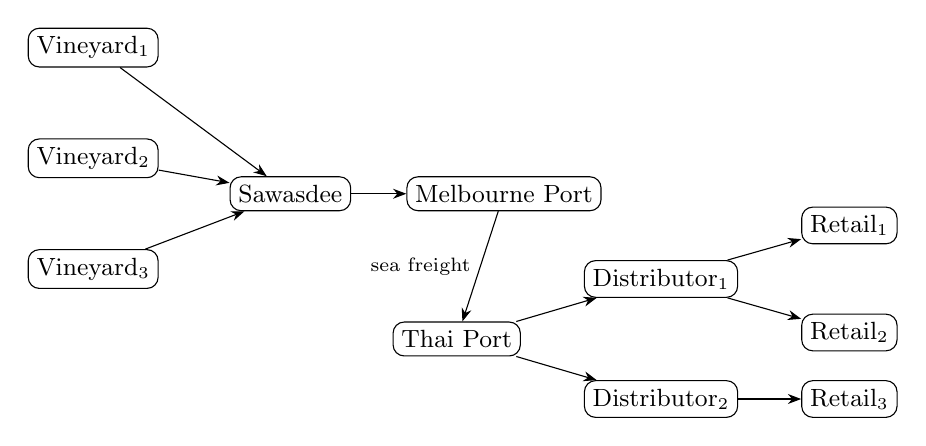
\begin{tikzpicture}[node distance=9mm and 9mm,
  every node/.style={font=\small},
  fac/.style={draw, rounded corners, inner sep=3pt},
  arr/.style={-{Stealth}}]
\node[fac] (T) {Vineyard$_1$};
\node[fac, below=of T] (U) {Vineyard$_2$};
\node[fac, below=of U] (H) {Vineyard$_3$};
\node[fac, right=of U, yshift=-4.5mm] (W) {Sawasdee};
\node[fac, right=7mm of W] (PA) {Melbourne Port};
\node[fac, below=14mm of PA, xshift=-6mm] (LC) {Thai Port};
\node[fac, above right=3mm and 8mm of LC] (S) {Distributor$_1$};
\node[fac, below right=3mm and 8mm of LC] (L) {Distributor$_2$};
\node[fac, above right=2mm and 8mm of S] (M1) {Retail$_1$};
\node[fac, below right=2mm and 8mm of S] (M2) {Retail$_2$};
\node[fac, right=8mm of L] (M3) {Retail$_3$};
\draw[arr] (T) -- (W);
\draw[arr] (U) -- (W);
\draw[arr] (H) -- (W);
\draw[arr] (W) -- (PA);
\draw[arr] (PA) -- (LC) node[midway, left, font=\scriptsize]{sea freight};
\draw[arr] (LC) -- (S);
\draw[arr] (LC) -- (L);
\draw[arr] (S) -- (M1);
\draw[arr] (S) -- (M2);
\draw[arr] (L) -- (M3);
\end{tikzpicture}

\end{center}

The model above is everything a pure \emph{distributor} needs:
nothing is manufactured, everything is bought finished, and goods
keep their identity from vineyard to shelf. Notice also that the
shipping graph is a \emph{tree}: the first rung of the ladder.
Sections \ref{sec:network} and \ref{sec:steel} stay on that rung;
Sections \ref{sec:dag} and \ref{sec:graph} climb.

%% ============================================================
\section{Glossary: Supply-Chain Terms}\label{sec:glossary}

Supply chain management has its own vocabulary, standardized by decades
of industry practice. This section collects the terms used in this
note, aimed at a reader who knows what a comonad is but not what a
duty point is.

\begin{description}[nosep]
\item[Markup / margin.] The percentage a tier adds when goods change
  hands: the difference between what it pays and what it charges.
  Margins compound multiplicatively along a route---each hand-off
  applies $\times(1+m)$---and enter the fiscal stack at a definite
  point (Section~\ref{sec:tracking}).

\item[Landed cost.] The full cost of goods delivered at a
  destination: purchase price plus freight, insurance, duties, and
  taxes. In Section~\ref{sec:tracking} it is the value of a composite
  affine map applied to the ex-cellar price.

\item[Sourcing.] The assignment of a producer to each thing that must
  be made or bought: \emph{which facility makes which component}.
  Section~\ref{sec:sourcing} makes this a functor.

\item[Facility.] Any node of the network through which goods pass:
  vineyard, port, distributor, retailer. A facility need not be a
  physical place that holds stock---Sawasdee itself is an agency,
  a node where goods change \emph{custody and price} but never
  sit on a shelf. Legal nodes and physical nodes enter the network
  on equal terms (compare the bonded warehouse, below).

\item[Shipping leg / route.] A leg is a single direct movement
  capability between two facilities; a route is a composable sequence
  of legs. Legs generate, routes compose: Section~\ref{sec:network} takes the free
  category.

\item[Distributor / distribution centre.] A facility that holds
  finished goods close to customers and ships only
  downstream---toward retail, never back into production
  (Distributor$_1$ in Bangkok and Distributor$_2$ in Chiang Mai, in
  our example).

\item[Last mile.] The final delivery leg, from the last stocking
  point to the customer or retailer. The shortest legs of the network
  and collectively the most expensive---typically $40$--$50\%$ of
  total logistics cost---because the trunk network's consolidation
  fans out into many small terminal shipments. For wine it must also
  be the last link of the cold chain
  (Section~\ref{sec:tracking}).

\item[Cold chain.] The requirement that a temperature-sensitive
  product stay within a temperature band along its \emph{entire}
  journey---refrigerated warehouses, insulated or actively cooled
  (``reefer'') containers, and controlled handoffs between them. One
  breach anywhere spoils the whole chain
  (Section~\ref{sec:tracking}).

\item[Tariff / customs duty.] A tax levied when goods cross a border.
  A \textbf{specific} duty is a fixed amount per unit; an \textbf{ad
  valorem} duty is a percentage of declared value. They accumulate
  along a route additively and multiplicatively respectively
  (Section~\ref{sec:tracking}).

\item[Excise; duty point.] A tax on certain goods (alcohol among
  them) triggered not by movement but by an event: the \textbf{duty
  point}, typically release into home consumption. Until then goods
  can move and be stored \emph{in bond}, duty-unpaid
  (Remark~\ref{rem:dutypoint}).

\item[Bonded warehouse.] A warehouse authorized by customs to hold
  goods with duty suspended. A facility distinguished by legal
  status, not physical function---the same building, bonded or
  duty-paid, is two different nodes for planning purposes.

\item[Consolidation.] The gathering of goods from several origins
  into one shipment rather than shipping each separately: bottles
  from three vineyards meet in one export container. In
  Section~\ref{sec:sourcing} this is the functoriality of sourcing.

\item[Inventory.] The stock currently held at a facility, per
  product: a vector in $\mathbb{N}^{\Prod}$, where $\Prod$ is the
  set of distinct products handled. Modified by \textbf{receipts}
  (arrivals), \textbf{issues} (consumption or dispatch), and
  \textbf{transfers} (movements between facilities)---collectively,
  \emph{stock movements} (Section~\ref{sec:inventory}).

\item[Replenishment policy.] A rule that observes current stock and
  decides what to reorder, when, and how much. Section~\ref{sec:inventory} identifies
  such policies with Kleisli maps of an update monad.

\item[Lead time.] The total delay between deciding to order
  something and having it available: for an order placed on a
  vineyard, the time until the case is on the retail shelf. Along a
  fixed route it is the sum of the transit times of the legs---a
  tracking functor like any other (Section~\ref{sec:tracking}).

\item[Aggregate planning.] Planning done at a coarsened level---regions
  instead of facilities, product families instead of individual
  products, quarters
  instead of days---because demand is forecast and decisions are made
  coarse before they are executed fine. Section~\ref{sec:cofunctors} models the
  coarse-to-fine passage as a cofunctor.

\item[Demand fulfilment.] The process of turning expressed demand
  (``Thailand needs shiraz'') into concrete execution (specific
  facilities shipping along specific routes): the lifting problem of
  Section~\ref{sec:cofunctors}.

\item[Order book.] The ledger of outstanding orders not yet fulfilled:
  committed future stock movements, as opposed to inventory, which
  records their accumulated past effect (Section~\ref{sec:inventory}).

\item[Bullwhip effect.] Forrester's observation that the variance of
  orders \emph{amplifies} as one moves upstream, away from final
  demand: retailers see ripples, raw-material suppliers see waves.
  Each tier reacts to its neighbour's orders rather than to true
  demand, compounding delay and overcorrection (Section~\ref{sec:outlook}).
\end{description}

%% ============================================================
\section{Containers and Directed Containers}\label{sec:dcont}

We briefly recall the definitions
\cite{abbott-altenkirch-ghani, ahman-chapman-uustalu}.

\begin{definition}
A \textbf{container} $\cont{S}{P}$ consists of a set $S$ of
\textbf{shapes} and, for each shape $s$, a set $P(s)$ of
\textbf{positions}. Its \textbf{extension} is the functor
$\Ext{\cont{S}{P}} : \Set \to \Set$ given by
\[
\Ext{\cont{S}{P}}(X) \;=\; \sum_{s \in S} X^{P(s)},
\]
i.e.\ a shape together with an $X$-value at every position.
\end{definition}

Extensions of containers are exactly the polynomial functors in one
variable; in Spivak's notation \cite{spivak-poly, niu-spivak} one
writes $p = \sum_{s \in S} y^{P(s)}$ and works in the category $\Poly$.

\begin{definition}\label{def:dcont}
A \textbf{directed container} \cite{ahman-chapman-uustalu} is a
container $\cont{S}{P}$ equipped with:
\begin{itemize}[nosep]
\item a \textbf{subshape} operation: for $s \in S$ and $p \in P(s)$, a
  shape $s \dc p \in S$;
\item a \textbf{root} position $\obs_s \in P(s)$ for each $s$;
\item a \textbf{translation} operation: for $p \in P(s)$ and
  $p' \in P(s \dc p)$, a position $p \oplus p' \in P(s)$;
\end{itemize}
subject to five laws:
$s \dc \obs_s = s$;\quad
$s \dc (p \oplus p') = (s \dc p) \dc p'$;\quad
$p \oplus \obs = p$;\quad
$\obs \oplus p = p$;\quad
$(p \oplus p') \oplus p'' = p \oplus (p' \oplus p'')$.
\end{definition}

Two theorems make this structure important.

\begin{theorem}[Ahman--Chapman--Uustalu \cite{ahman-chapman-uustalu}]
Directed container structures on $\cont{S}{P}$ are exactly comonad
structures on $\Ext{\cont{S}{P}}$. The counit and comultiplication are
\[
\varepsilon(s, v) = v(\obs_s),
\qquad
\delta(s, v) = \bigl(s,\; \lambda p.\, (s \dc p,\; \lambda p'.\, v(p \oplus p'))\bigr).
\]
\end{theorem}

\begin{theorem}[Ahman--Uustalu \cite{ahman-uustalu-categories};
Spivak et al.\ \cite{niu-spivak}]
Directed containers are exactly small categories: shapes are objects,
$P(s)$ is the set of morphisms \emph{out of} $s$, the subshape
$s \dc p$ is the codomain of $p$, the root $\obs_s$ is the identity,
and $\oplus$ is composition. Equivalently, directed containers are the
comonoids in $(\Poly, \triangleleft, y)$.
\end{theorem}

\begin{slogan}
A directed container is a system of \emph{local views}: every shape
knows its positions, every position leads to a subshape with its own
positions, and the two levels of description agree. The comonad laws
\emph{are} this agreement.
\end{slogan}

Supply chains are full of local views---a warehouse's view of its
downstream network, a subassembly's view of its own components---and
this is why the language fits.

%% ============================================================
\section{Trees I: The Shipping Network as a Directed Container}\label{sec:network}

We first give the pure mathematics, with no supply chain in sight,
and only then interpret it.

\begin{construction}\label{con:network}
Let $G$ be a finite directed graph: a set $V$ of nodes and a set of
edges, each with a source and a target in $V$. The nodes are
\emph{labelled} in the combinatorialist's sense---$V$ is a set of
distinguishable elements, not an isomorphism class---and no node is
distinguished as a root. Define the directed container $\N = \N_G$:
\begin{itemize}[nosep]
\item \textbf{shapes}: nodes, $S = V$;
\item \textbf{positions}: $P(v)$ is the set of finite directed paths
  in $G$ starting at $v$, including the empty path;
\item $v \dc \rho$ is the node where the path $\rho$ ends;
\item $\obs_v$ is the empty path at $v$;
\item $\rho \oplus \rho'$ is concatenation: follow $\rho$, then
  continue along $\rho'$.
\end{itemize}
The five laws are immediate. As a category, $\N$ is the free category
on $G$.  In the formalization, the construction is
\texttt{Digraph.network} in \texttt{Network.lean}; each concrete graph
$G$ produces its own directed container $\N_G$.
\end{construction}

The construction accepts \emph{any} directed graph $G$. This
section works out what happens on the simplest kind.

\begin{proposition}\label{prop:tree}
If the underlying undirected graph of $G$ is a tree (such a $G$ is
called a \emph{polytree}), then $\N$ is \emph{thin}: between any
two nodes there is at most one path. Thus $\N$ is a poset, the
reachability order on nodes, and a position carries no more
information than its endpoint:
\[
P(v) \;\cong\; \{\text{nodes reachable from } v\}.
\]
\end{proposition}

\begin{proof}
Two distinct paths from $v$ to the same node would trace out a
cycle in the underlying undirected graph. So
$\rho \mapsto v \dc \rho$ is injective, and it is surjective onto
the reachable nodes by definition.
\end{proof}

$\N$ is exactly the directed container of a finite tree: shapes
are the nodes, and each node's positions are the nodes downstream
of it (itself included).

This pure structure maps directly onto the supply chain of
Section~\ref{sec:setup}, with nothing added and nothing forced:

\begin{center}
\begin{tabular}{ll}
\toprule
Pure structure & Supply-chain reading \\
\midrule
node of $G$ & facility \\
edge of $G$ & shipping leg \\
directed path & shipping route \\
empty path $\obs_f$ & goods staying at $f$ \\
endpoint $f \dc \rho$ & destination of the route \\
concatenation $\oplus$ & composition of routes \\
polytree hypothesis & the wine network's shape \\
\bottomrule
\end{tabular}
\end{center}

For Sawasdee Cellars: $P(\text{Vineyard}_1)$ has nine elements---the
empty route, and one route for each of the eight facilities reachable
from Vineyard$_1$: through Sawasdee and the Melbourne Port,
across the sea to the Thai Port, branching to the two distributors,
and fanning out to
the three retailers. $P(\text{Retail}_1)$ has only the empty route:
retail is the end of the line. Two kinds of leg deserve comment. The
\textbf{deep-sea leg} Melbourne Port${}\to{}$Thai Port is the longest:
ten days in a refrigerated (``reefer'') container. The final legs
from the distributors to the retailers---Distributor$_1$ to Retail$_1$
and Retail$_2$, Distributor$_2$ to Retail$_3$---are the \textbf{last mile}:
refrigerated van deliveries, the shortest legs of the network and the
only ones the customer ever sees. They are legs like any other---but
each is the last link of the cold chain, and by idempotence of $\max$
(Section~\ref{sec:tracking}) a single warm van undoes the
refrigerated integrity of the entire route from the vineyard. In
Bangkok, at $35^{\circ}$C ambient, emphatically so.

Note that the tree has no marked root---and could not be given
one. In a rooted tree the root does real work: it orients every
edge away from itself, so each node has at most one leg in. Here
Sawasdee, with three legs in and one out, is not a root but the
\emph{waist} of the network, through which every bottle's title
passes; no choice of root generates this orientation, which comes
from the flow of goods instead. Nor does the theory miss a root: a
directed container has a \emph{local} root $\obs_f$ at every
shape---each facility is the root of its own downstream view.
Rooted trees will appear in Section~\ref{sec:steel}, used in the
opposite way: there each entire rooted tree is a single
\emph{shape}, and the root is essential data---the product being
made. Distribution has no privileged vantage point; manufacture
has a privileged product.

An element of $\Ext{\N}(X)$ is a facility $f$ together with an
$X$-value on every route out of $f$: a \textbf{decorated downstream
view}. Take $X = \mathbb{R}$ and decorate each route with its transit
time; or take $X = \{\text{ok}, \text{delayed}, \text{blocked}\}$ and
decorate each route with its status.

The comonad structure is where the interpretation earns its keep:
\begin{itemize}[nosep]
\item The counit $\varepsilon$ reads the value at the empty route:
  \emph{look at your own facility}.
\item The comultiplication $\delta$ sends a decorated view at $f$ to a
  view-of-views: each route $\rho$ out of $f$ is decorated with the
  \emph{entire downstream view of the facility at the end of $\rho$},
  obtained by reading $f$'s original decoration along composite routes
  $\rho \oplus \rho'$.
\end{itemize}

\begin{slogan}\label{slo:coherence}
The comonad laws say that Sawasdee's view of the Thai Port, as
computed from within Vineyard$_1$'s view, equals the Thai Port's own
view. Supply chain visibility is comonadic coherence.
\end{slogan}

\subsection{Tracking along routes: cold chain, tariffs, markups, compliance}
\label{sec:tracking}

Wine export lives under constant surveillance: temperature must stay
in range, duties and taxes accrue at borders, every intermediary adds
its margin, every leg needs the right licences. All of these are
instances of one construction.

\begin{construction}\label{con:tracking}
Let $(M, \oplus, e)$ be a monoid, regarded as a one-object
category $\mathbf{B}M$. A \textbf{compositional tracking} of $M$-data
is a functor $d : \N \to \mathbf{B}M$: an assignment of $d(\rho) \in M$
to every route, satisfying
\[
d(\obs_f) = e, \qquad d(\rho \oplus \rho') = d(\rho) \oplus d(\rho').
\]
Since $\N$ is free on the shipping graph $G$---every route is a
composite of legs, and distinct sequences of legs are distinct
routes, with no equations between them---such a functor is
\emph{exactly} a labelling of individual legs: measure per leg, and
the functor computes per route. Audit locally, certify globally---that
is the universal property of the free category.
\end{construction}

On a tree (Proposition~\ref{prop:tree}) this is especially concrete:
a tracking is an edge-labelling of the tree, composed along the
unique path between any two facilities.

The choice of monoid is the choice of what is being tracked:
\begin{center}
\begin{tabular}{lll}
\toprule
Tracked quantity & Monoid & Character \\
\midrule
freight cost, specific duty & $(\mathbb{R}_{\geq 0}, +, 0)$ & extensive \\
ad valorem tariff, markup & $(\mathbb{R}_{> 0}, \times, 1)$ & multiplicative \\
peak temperature & $(\mathbb{R} \cup \{-\infty\}, \max, -\infty)$ & path-critical \\
cold chain intact? & $(\{\mathrm{ok}, \mathrm{broken}\}, \wedge, \mathrm{ok})$ & idempotent \\
licences required & $(\mathcal{P}(L), \cup, \emptyset)$ & accumulative \\
price build-up & $(\mathrm{Aff}, \circ, \mathrm{id})$ & order-sensitive \\
\bottomrule
\end{tabular}
\end{center}

\begin{itemize}[nosep]
\item \textbf{Taxes and tariffs.} Specific duties (baht per case)
  add along a route; ad valorem duties (a percentage of value)
  compose multiplicatively. Both are functors; only the target monoid
  differs. A leg that crosses no border is labelled $e$.
\item \textbf{Markups.} Wine changes hands at each tier: vineyard to
  Sawasdee, Sawasdee to distributor, distributor to retailer. Each
  hand-off applies a margin $\times(1+m)$; label each leg with the
  margin taken at its source, and the functor into
  $(\mathbb{R}_{>0}, \times, 1)$ compounds them. The gap between
  ex-cellar price and Bangkok shelf price is a composite morphism.
\item \textbf{Cold chain.} Peak temperature composes by $\max$---an
  \emph{idempotent} monoid, which is precisely the formal content of
  ``chain'': a single hot hour on the wharf dominates ten cold days at
  sea, and no subsequent refrigeration composes it away. The composite
  is as good as its worst morphism.
\item \textbf{Licences and regulatory compliance.} Let $L$ be the set
  of permits: export licences, import licences, alcohol distribution
  licences, organic and appellation certifications. The functor
  $d : \N \to \mathbf{B}(\mathcal{P}(L))$ assigns each route the set of
  licences it requires---the union over its legs. An operator holding
  licence set $A \subseteq L$ may lawfully use route $\rho$ iff
  $d(\rho) \subseteq A$. Compliance checking is a subset test against
  a functorially aggregated requirement.
\item \textbf{Price build-up: landed cost and shelf price.} The full
  pricing rule mixes multiplicative pieces (margins, ad valorem duty,
  VAT) with additive ones (freight per case, specific duty, excise).
  Neither monoid alone suffices. The natural target is the monoid
  $\mathrm{Aff}$ of affine maps $v \mapsto av + b$ ($a > 0$, $b \geq 0$)
  under composition: label each leg with the affine map its hand-off
  applies, and the composite $d(\rho) \in \mathrm{Aff}$ turns an
  ex-cellar price into a price at the end of the route,
  $v \mapsto d(\rho)(v)$.
\end{itemize}

\begin{remark}\label{rem:noncommutative}
$\mathrm{Aff}$ is \emph{not} commutative, and this is a feature, not a
defect: a $10\%$ margin applied before a specific excise of $b$ baht
differs from the same margin applied after it, by exactly
$b/10$. Statutory stacking rules are order-sensitive---Thai customs
duty is assessed on the CIF value, excise on top of that, VAT on the
duty- and excise-inclusive value, local taxes on top again, and each
tier's margin enters at its own point in the chain. Legs of a route
occur in a definite order; the free category remembers that order;
and a functor $d : \N \to \mathbf{B}\mathrm{Aff}$ maps the order of
hand-offs to the order of function composition. Commutative
trackings are the special case where the bookkeeping may be done in
any order---the fiscal ones may not. (On the Australian side the
stack is short: exports are free of GST and of WET, the wine
equalisation tax, so the legs up to the Melbourne Port carry only
freight and margin.)
\end{remark}

Each tracking functor generates decorated views: the assignment
$f \mapsto (\rho \mapsto d(\rho))$ is an element of $\Ext{\N}(M)$ over
every shape at once, and Slogan~\ref{slo:coherence} applies verbatim:
Vineyard$_1$'s record of duties and temperatures beyond Sawasdee
agrees with Sawasdee's own record. Traceability---the auditable
handoff between successive custodians that customs and insurers
demand---is comonadic coherence.

\begin{remark}\label{rem:dutypoint}
One compliance notion resists this pattern: \emph{excise}. Excise duty
is not accrued along a route but triggered by an event---release from
bond, the \emph{duty point}. A bonded warehouse and a duty-paid
warehouse may be the same building in different legal states. Tracking
state changed by events is the update-monad side of the theory, taken
up in Section~\ref{sec:inventory}; the duty point is a stock movement
in a fiscal, not physical, dimension.
\end{remark}

%% ============================================================
\section{Trees II: Bills of Materials---Steel}\label{sec:steel}

Everything so far ran on a single directed container, the network
$\N$, and that was enough for a reason worth stating: Sawasdee
Cellars is a pure \emph{distributor}. A bottle leaving Vineyard$_1$
is the same bottle on the Bangkok shelf; the network moves goods but
never transforms them, so one ontology---facilities and
routes---suffices, and every compliance question is route-borne. To
see what manufacturing adds, we change examples: \emph{Falcon
Steel}, a producer in Abu Dhabi's Mussafah industrial area, making
reinforcing bar (rebar) for export.

The pipeline is gas-based, as is standard in the Gulf. Imported
\textbf{iron ore pellets} arrive at the ore berth and are reduced to
\textbf{DRI} (direct reduced iron) at a reduction plant; the melt
shop melts DRI together with \textbf{scrap} in an electric arc
furnace and casts \textbf{billets}; the rolling mill rolls billets
into \textbf{rebar}, which leaves through Khalifa Port for two
overseas distributors---one in Rotterdam serving EU construction,
one in Dammam serving the Gulf:

\begin{center}
\begin{tabular}{lll}
\toprule
Facility & Location & Role \\
\midrule
Ore Berth & Mussafah & receives imported pellets \\
Reduction Plant & Mussafah & reduces pellets to DRI (gas) \\
Melt Shop & Mussafah & EAF; melts DRI + scrap, casts billets \\
Rolling Mill & Mussafah & rolls billets into rebar \\
Khalifa Port & Abu Dhabi & container port \\
Distributor$_{\mathrm{EU}}$ & Rotterdam & EU distributor \\
Distributor$_{\mathrm{GCC}}$ & Dammam & Gulf distributor \\
\bottomrule
\end{tabular}
\end{center}

The shipping graph:

\begin{center}
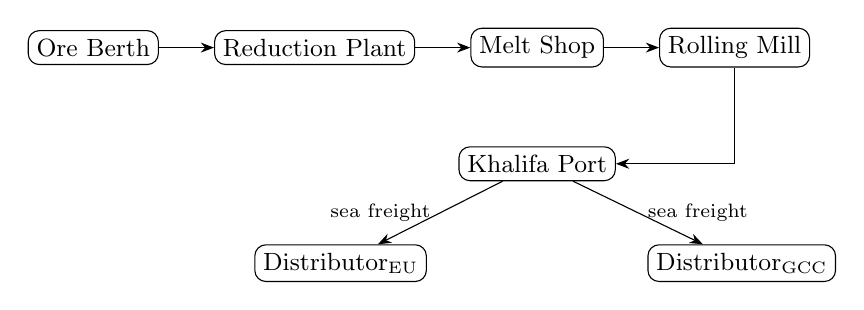
\begin{tikzpicture}[node distance=8mm and 7mm,
  every node/.style={font=\small},
  fac/.style={draw, rounded corners, inner sep=3pt},
  arr/.style={-{Stealth}}]
\node[fac] (O) {Ore Berth};
\node[fac, right=of O] (R) {Reduction Plant};
\node[fac, right=of R] (M) {Melt Shop};
\node[fac, right=of M] (RM) {Rolling Mill};
\node[fac, below=10mm of M] (P) {Khalifa Port};
\node[fac, below left=8mm and 4mm of P] (EU) {Distributor$_{\mathrm{EU}}$};
\node[fac, below right=8mm and 4mm of P] (GCC) {Distributor$_{\mathrm{GCC}}$};
\draw[arr] (O) -- (R);
\draw[arr] (R) -- (M);
\draw[arr] (M) -- (RM);
\draw[arr] (RM) |- (P);
\draw[arr] (P) -- (EU) node[midway, left, font=\scriptsize]{sea freight};
\draw[arr] (P) -- (GCC) node[midway, right, font=\scriptsize]{sea freight};
\end{tikzpicture}
\end{center}

This graph is a directed container exactly as in
Construction~\ref{con:network}: call it $\N_{\mathrm{steel}}$, a
second instance of the \emph{same} construction on a different graph
(the wine network $\N$ was the first; in the formalization both are
the one definition \texttt{network} of \texttt{Network.lean} applied
to two concrete graphs, with \texttt{Steel.graph} in
\texttt{Sourcing.lean} covering the four production facilities). The
underlying undirected graph is again a tree---a spine with one
fan-out at the port---so Proposition~\ref{prop:tree} applies:
$\N_{\mathrm{steel}}$ is thin, and $P(\text{Ore Berth})$ has seven
elements, the empty route plus one route to each facility
downstream; $P(\text{Distributor}_{\mathrm{EU}})$ has one. Every
tracking functor of Section~\ref{sec:tracking} applies verbatim,
though the monoids that carry weight have changed with the industry:
\begin{itemize}[nosep]
\item \textbf{Duties.} The EU leg attracts a safeguard or
  anti-dumping duty, ad valorem: $(\mathbb{R}_{>0}, \times, 1)$.
  Freight and specific duties add in $(\mathbb{R}_{\geq 0}, +, 0)$.
\item \textbf{Certificates.} A rebar consignment travels with its
  \textbf{mill test certificate} (EN 10204 type 3.1, attesting
  chemistry and mechanical properties) and its certificate of
  origin: $(\mathcal{P}(L), \cup, \emptyset)$, exactly the licence
  functor of the wine network with a different $L$.
\item \textbf{What is absent.} Steel needs no cold chain; the
  idempotent monoid sits unused. Its path-critical role reappears as
  $(\max, +)$ lead time in Section~\ref{sec:rollups}.
\end{itemize}
A path with a fan-out is a tree, so we have not yet left the
first rung. What \emph{is} new is
that goods now change identity: pellets are consumed and DRI
appears; the product on a facility's outbound leg is not the product
on its inbound leg. The document recording these identity changes is
the \textbf{bill of materials} (BOM): the recursive parts list of a
manufactured product---the direct components needed to make one
unit, each component carrying its own BOM. Manufactured components
(the billet) are called \textbf{subassemblies}; raw materials and
purchased goods (ore pellets, scrap) are the leaves. Purchasing,
costing, and scheduling all read from this document:

\begin{center}
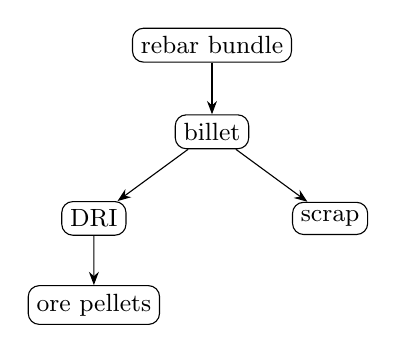
\begin{tikzpicture}[
  every node/.style={font=\small, draw, rounded corners, inner sep=3pt},
  edge from parent/.style={draw, -{Stealth}},
  level distance=11mm, sibling distance=30mm]
\node {rebar bundle}
  child {node {billet}
    child {node {DRI}
      child {node {ore pellets}}}
    child {node {scrap}}};
\end{tikzpicture}
\end{center}

\subsection{Bills of materials as a directed container}\label{sec:bom}

\begin{construction}\label{con:bom}
A \textbf{BOM tree} is a finite rooted tree whose nodes are labelled
by products: the children of a node are the direct components of one
unit of it. Define the directed container
$\B$:
\begin{itemize}[nosep]
\item \textbf{shapes}: BOM trees;
\item \textbf{positions}: $P(t)$ is the set of \textbf{occurrences}
  in $t$---descending paths from the root, including the empty path;
\item $t \dc p$ is the subtree at $p$: the occurrence's own BOM;
\item $\obs_t$ is the empty occurrence: the product itself;
\item $p \oplus p'$ is path concatenation: an occurrence inside a
  component, seen from the finished product.
\end{itemize}
The five laws are immediate: $\B$ is the directed container of
rooted trees, with positions the paths---a second directed
container, living beside---not on---the network; its
shapes are documents, not facilities. In the formalization it is
\texttt{bom} in \texttt{Sourcing.lean} (a separate construction from
\texttt{Digraph.network}; a different directed container, not another
application of $\N_{(-)}$), whose shapes additionally
carry the routing choices needed by
Construction~\ref{con:sourcing} below (see
Section~\ref{sec:formalization}).
\end{construction}

Concretely, Falcon Steel's rebar BOM drawn above has five
occurrences:
\[
\langle\rangle,\quad
\text{billet},\quad
\text{billet}\cdot\text{DRI},\quad
\text{billet}\cdot\text{scrap},\quad
\text{billet}\cdot\text{DRI}\cdot\text{ore},
\]
the empty occurrence being the rebar itself. Note the shift of
ontology between the two containers: in $\N_{\mathrm{steel}}$ a
position at a shape is a route \emph{out of a facility}; in $\B$ it
is a place \emph{inside a document}. And where
Section~\ref{sec:network} argued that the shipping tree has no root
and could not be given one, here the root is essential data: a BOM
tree without its root product is not a parts list of anything.

The comonad structure translates industry practice directly. The
counit reads the value at the empty occurrence: \emph{look at the
product itself}. The comultiplication decorates every occurrence
with the entire sub-BOM below it---which is precisely what
material requirements planning (MRP) software calls \textbf{BOM
explosion}.

\begin{slogan}
BOM explosion is comultiplication. The comonad law
$s \dc (p \oplus p') = (s \dc p) \dc p'$ says the billet's parts
list, read off from within the rebar's exploded view, equals the
billet's own parts list---multi-level costing is coherent.
\end{slogan}

An element of $\Ext{\B}(X)$ is a BOM with an $X$-value at every
occurrence: unit cost, weight, production time, embedded carbon.

\subsection{Sourcing as a functor}\label{sec:sourcing}

Each product is made or received somewhere:

\begin{center}
\begin{tabular}{lll}
\toprule
Product & Facility & \\
\midrule
ore pellets & Ore Berth & received at the berth \\
DRI & Reduction Plant & made \\
scrap & Melt Shop & bought at the gate \\
billet & Melt Shop & made \\
rebar & Rolling Mill & made \\
\bottomrule
\end{tabular}
\end{center}

Write $\site(t)$ for the facility producing the
root product of the tree $t$.

\begin{construction}\label{con:sourcing}
Sourcing extends to a functor
$\site : \B \to \N_{\mathrm{steel}}^{\mathrm{op}}$:
\begin{itemize}[nosep]
\item on shapes, $t \mapsto \site(t)$;
\item an occurrence $p \in P(t)$ is sent to a chosen \textbf{inbound
  route} in $\N_{\mathrm{steel}}$ from $\site(t \dc p)$ to
  $\site(t)$: the route the component travels to its point of use.
\end{itemize}
The $(-)^{\mathrm{op}}$ is forced by orientation: positions of $\B$
point \emph{down} the parts tree, from product to component, while
goods flow \emph{up} it, from component to product---an occurrence
out of $t$ becomes a route \emph{into} $\site(t)$. Functoriality
says the empty occurrence is sourced by the empty route, and the
route for a nested occurrence is the composite through the
intermediate producer: ore reaches the rolling mill only via the
reduction plant and the melt shop, changing identity at each stop.
\textbf{Consolidation}---components gather where their parent is
made---is exactly the functor laws.
\end{construction}

Worked through for Falcon Steel's deepest occurrence: the chosen
inbound leg for each BOM edge is the single shipping leg from the
component's producer to its parent's producer, and the ore
occurrence $\text{billet}\cdot\text{DRI}\cdot\text{ore}$ factors as
$(\text{billet}\cdot\text{DRI}) \oplus \text{ore}$, so
functoriality forces
\[
\site(\text{billet}\cdot\text{DRI}\cdot\text{ore})
=
\underbrace{(\text{Berth} \to \text{Reduction})}_{\text{ore, within DRI's BOM}}
\oplus
\underbrace{(\text{Reduction} \to \text{Melt} \to \text{Mill})}_{\text{DRI, within rebar's BOM}},
\]
the three-leg journey of the ore, read off from the parts list: the
component's own journey first, then its subassembly's. This is the
consolidation equation checked by \texttt{rfl} in the
formalization.

In the formalization, the two containers of this section and the
functor between them are all in \texttt{Sourcing.lean}: $\B$ is
\texttt{bom}, $\N_{\mathrm{steel}}^{\mathrm{op}}$ is
\texttt{network graph.op} (reversing the graph rather than opposing
the category), and $\site$ is \texttt{sourcing}, with
\texttt{DContFunctor.lean} supplying the notion of covariant functor
of directed containers. The rebar tree drawn above, ore's three-leg
inbound route to the rolling mill, and one consolidation equation
are all checked definitionally (\texttt{rfl}).

\subsection{Roll-ups, and compliance on two containers}\label{sec:rollups}

A \textbf{roll-up} aggregates per-component data to the product
level. For data valued in a commutative monoid---unit costs in
$(\mathbb{R}_{\geq 0}, +, 0)$, weights likewise---the roll-up is the
sum over all occurrences of the BOM tree. Lead time is subtler: over
each root-to-leaf path one \emph{adds} production and transit times,
then takes the \emph{maximum} over paths---the critical path, living
in the $(\max, +)$ semiring rather than a single monoid. The general
theory of such aggregations is worked out by Spivak, Garner, and
Fairbanks \cite{spivak-aggregation}.

For Falcon Steel the cost roll-up is a five-line sum: decorate each
occurrence of the rebar BOM with the cost \emph{added} there---the
element of $\Ext{\B}(\mathbb{R}_{\geq 0})$ a standard costing run
produces---and sum over occurrences (illustrative figures, per tonne
of rebar):

\begin{center}
\small
\begin{tabular}{llr}
\toprule
Occurrence & Cost added & \$/t \\
\midrule
$\langle\rangle$ (rebar) & rolling conversion & 70 \\
billet & melt + cast conversion & 90 \\
billet$\cdot$DRI & reduction conversion & 60 \\
billet$\cdot$scrap & scrap purchase & 80 \\
billet$\cdot$DRI$\cdot$ore & pellet purchase & 140 \\
\midrule
roll-up & sum over $P(t)$ & 440 \\
\bottomrule
\end{tabular}
\end{center}

The \emph{rolled-up cost of the billet alone} is the same sum over
the sub-BOM $t \dc \text{billet}$---and the coherence law of
Slogan~\ref{slo:coherence}'s BOM analogue (Section~\ref{sec:bom})
says computing it inside the rebar's exploded view or from the
billet's own parts list must agree: $90 + 60 + 80 + 140 = 370$
either way. Multi-level costing is coassociativity, with arithmetic.

The most instructive compliance case lives on \emph{both} containers
at once. The EU's carbon border adjustment mechanism (CBAM) requires,
at the border, one number: total embedded CO$_2$ per tonne of rebar.
That number is assembled from a decoration of $\B$ (the emissions of
each production step, at each occurrence) plus a tracking on
$\N_{\mathrm{steel}}$ (the emissions of each shipping leg, as in
Construction~\ref{con:tracking}), the two glued along $\site$: each
occurrence contributes its process emissions and the emissions of its
inbound route (illustrative figures, per tonne of rebar):

\begin{center}
\small
\begin{tabular}{llrlr}
\toprule
Occurrence & Process step & t\,CO$_2$/t & Inbound route ($\site$) & t\,CO$_2$/t \\
\midrule
$\langle\rangle$ (rebar) & rolling & 0.10 & --- & --- \\
billet & EAF melt + cast & 0.35 & Melt $\to$ Mill & 0.01 \\
billet$\cdot$DRI & gas reduction & 0.70 & Reduction $\to$ Melt $\to$ Mill & 0.02 \\
billet$\cdot$scrap & gate processing & 0.02 & Melt $\to$ Mill & 0.01 \\
billet$\cdot$DRI$\cdot$ore & pelletizing (upstream) & 0.15 & Berth $\to \cdots \to$ Mill & 0.03 \\
\midrule
total & & 1.32 & & 0.07 \\
\bottomrule
\end{tabular}
\end{center}

Roughly $1.4$ t\,CO$_2$ per tonne of rebar---a single auditable
figure, computed from two directed containers and the functor
connecting them, and the reason the computation is commercially
live: the gas-DRI route sits well below the blast-furnace route's
$\approx 2.2$, and CBAM prices exactly that difference. One boundary
subtlety is also structural: the deep-sea leg to Rotterdam is
tracked in the same monoid but sits outside CBAM's system
boundary---the regulation selects a \emph{sub-tracking}, not a new
construction.

\begin{remark}[What the second example buys]
The dividing line between the two examples is now sharp. As long as
goods keep their identity along every morphism---distribution---one
directed container suffices and all compliance is route-borne. The
moment goods merge, split, or change identity---manufacture---a
second directed container is forced, together with a functor
connecting the two ontologies. When aggregation and demand enter
(Section~\ref{sec:cofunctors}), sourcing will supply a second
family of compatibility squares alongside the tracking ones.
\end{remark}

%% ============================================================
\section{DAGs: Alternative Routes and Repeated Components}\label{sec:dag}

Neither Construction~\ref{con:network} nor
Construction~\ref{con:bom} used the tree property; only
Proposition~\ref{prop:tree} did. So let the graph $G$ be merely
directed and \emph{acyclic}. The free category on $G$ still has
every $P(v)$ finite and no nontrivial endomorphisms, but it is no
longer thin: two nodes may now be joined by several paths, and a
position carries strictly more information than its endpoint. That
is the entire content of this rung, and it is the pure statement
of a supply-chain fact: positions are \emph{routes}, not
destinations. Every construction above applies unchanged.

Both examples climb to this rung---each producing a new directed
container $\N_{G'}$ from a new graph $G'$---each for its own reason.

\emph{Wine: alternative routings.} Add one alternative
routing---transshipment via Singapore alongside the direct
sailing---and the new directed container $\N_{G'}$ (in the
formalization, \texttt{Digraph.network G'} in \texttt{Rungs.lean}) has
two routes from the Melbourne Port to the
Thai Port with the same endpoints but different peak temperature,
freight, and duty. It is precisely the tracking functors of
Section~\ref{sec:tracking} that force the two positions apart: a
functor out of $\N$ assigns its data per \emph{route}, and the
direct sailing and the transshipment disagree in every column of
the monoid table.

\emph{Steel: repeated components.} A billet needing two charges of
DRI has two DRI-edges in its BOM tree: two distinct positions of
$\B$ with the same subshape---the same product-labelled
tree---two occurrences of the same component, which may have
different suppliers, different mill certificates, different
embedded carbon. This can never happen in the network, whose
nodes are facilities and occur once each; it happens in the BOM
because its nodes are merely \emph{labelled} by products, and
labels may repeat. So $\B$ fails to be thin
for a manufacturing reason rather than a routing one: not several
routes between fixed endpoints, but several occurrences of one
component in one product.

%% ============================================================
\section{Graphs: Cycles and the Scrap Loop}\label{sec:graph}

Finally, drop acyclicity: let $G$ be an arbitrary finite directed
graph. A cycle in $G$ gives paths that loop, so in the directed
container $\N_G$ the free category
acquires nontrivial endomorphisms $v \to v$, and $P(v)$
becomes infinite---one path per number of laps
(in the formalization, \texttt{Digraph.network G\_scrap} in
\texttt{Rungs.lean}). Nothing in
Definition~\ref{def:dcont} minds: no finiteness and no acyclicity
was ever assumed. That is the pure mathematics of this rung; the
supply-chain reading is that a route may revisit a facility, and a
tracking functor prices the laps like any other composite.

The steel network genuinely lives on this rung. Every mill produces
\emph{home scrap}---cobbles and offcuts from the rolling
mill---which returns to the melt shop and is remelted. This is a
leg rolling mill${}\to{}$melt shop closing a loop, and a tracking
functor prices $n$ remelt passes as the $n$-fold composite: yield
loss multiplies, energy adds.

The BOM, however, remains a tree, and we can now say why rather
than decree it: \emph{scrap is a leaf of $\B$ because the parts
list cuts the cycle}. Costing treats returning scrap as a purchased
input, not as ``made of rebar, which is made of billet, which is
made of scrap, \dots''---the well-foundedness of the BOM is an
accounting decision, and it is exactly what keeps explosion
(comultiplication) terminating while the network loops freely.

One more inhabitant of this rung is still to come: the inventory
container of Section~\ref{sec:inventory}, in which a receipt
followed by an equal issue is already an endomorphism of the stock
state.

Acyclicity, like thinness, is a property of examples, never a
hypothesis of the theory.

%% ============================================================
\section{Aggregation and Demand: Cofunctors}\label{sec:cofunctors}

Functors are not the only structure-preserving maps between directed
containers. A morphism of directed containers in the sense of
Ahman--Uustalu maps shapes \emph{forward} and positions
\emph{backward}---this is precisely a \textbf{cofunctor} (also called
a retrofunctor) \cite{aguiar, clarke-di-meglio}.

\begin{definition}
A cofunctor $\Phi : \mathcal{C} \nrightarrow \mathcal{D}$ consists of
a map $\varphi : \mathrm{Ob}\,\mathcal{C} \to \mathrm{Ob}\,\mathcal{D}$
together with, for each object $c$ and each morphism
$g : \varphi(c) \to d$ in $\mathcal{D}$, a chosen \textbf{lift}
$\Phi_c(g) : c \to c_g$ in $\mathcal{C}$ with $\varphi(c_g) = d$,
preserving identities and composition.
\end{definition}

\begin{construction}\label{con:aggregation}
Let $\widetilde{\N} = \N_{\widetilde{G}}$ be the \textbf{aggregate network}---yet another
application of Construction~\ref{con:network}, this time to a two-node
graph $\widetilde{G}$: shapes are
regions or tiers (say \emph{Australia} and \emph{Thailand}, with a
single leg from Australia to Thailand),
positions are aggregate routes
(in the formalization, \texttt{Digraph.network GAgg} in
\texttt{Aggregation.lean}). A \textbf{routing policy} is a
cofunctor $\Phi : \N \nrightarrow \widetilde{\N}$:
\begin{itemize}[nosep]
\item on shapes, each facility is assigned its region: $\varphi$
  sends the vineyards and every Australian facility (through
  the Melbourne Port) to Australia, and the Thai Port, the
  distributors, and the retailers to Thailand;
\item the lifting says: given a facility $f$ and an \emph{aggregate}
  route out of $\varphi(f)$---``move from Australia to
  Thailand''---the policy produces a \emph{concrete} route out
  of $f$ landing in the required region: from Sawasdee, the two legs
  Sawasdee${}\to{}$Melbourne Port${}\to{}$Thai Port; from
  Vineyard$_1$, the full route via Sawasdee. A single aggregate leg
  may lift to a many-leg concrete route---coarsening hides length,
  and the lift restores it.
\end{itemize}
The cofunctor laws say the policy is coherent: lifting an aggregate
identity does nothing, and lifting a composite aggregate route agrees
with lifting it in stages.
\end{construction}

This is the mathematical shape of \textbf{demand fulfilment}. Demand
is expressed at the aggregate level (``Thailand needs shiraz from
Australia''); execution happens at the concrete level (specific facilities,
specific routes). Planning systems are, structurally, machines for
lifting coarse morphisms to fine ones---cofunctors.

\begin{slogan}
Goods flow along functors; demand flows along cofunctors. A functor
pushes structure in the direction of its object map; a cofunctor pushes
objects forward but pulls the instructions backward.
\end{slogan}

\subsection{The two flows do not merge}

It is tempting to look for a single category of ``supply chain maps''
containing both sourcing functors and routing cofunctors. The
temptation should be resisted---and the literature agrees. Functors
and cofunctors between fixed categories are genuinely different
things, and neither subsumes the other. What exists instead is a
\textbf{double category}: functors in one direction, cofunctors in the
other, with squares expressing their compatibility. Clarke and
Di Meglio study this double category of functors and retrofunctors
\cite{clarke-di-meglio}; Fairbanks, Carlson, and Spivak
\cite{fairbanks-carlson-spivak} recover it from the general theory of
comonads, as the double category of polynomial comonads on $\Set$.

For Sawasdee Cellars, a square in this double category relates: a
tracking functor at the detailed level (duty, temperature, margin per
leg, as in Section~\ref{sec:tracking}), the corresponding tracking at
the aggregate level (total duty for the single leg
Australia${}\to{}$Thailand), and the routing policies connecting the
two levels---asserting that \emph{aggregate compliance is consistent
with per-leg compliance}: certifying the aggregate leg means
certifying whichever concrete route the policy lifts it to. That such
consistency is a square condition, not a commutation of two maps of
the same kind, is the deepest structural fact this note has to offer:
the disagreement between the two flows is preserved, not resolved.

Sourcing (Section~\ref{sec:sourcing}) supplies a second family of
squares of the same shape: a square relating detailed sourcing,
aggregate sourcing (``rebar is made in the Emirates and sold in
Europe''), and the routing policies connecting the two
levels---aggregate planning consistent with detailed execution.

%% ============================================================
\section{Inventory as an Update Monad}\label{sec:inventory}

Directed containers whose position sets are constant---$P(s) = M$ for
every shape $s$---are exactly \textbf{monoid actions}: $M$ is a monoid
(unit $\obs$, multiplication $\oplus$) acting on the set of shapes by
$s \dc m$. This is a third construction of directed containers,
distinct from both $\N_{(-)}$ and $\B$
(in the formalization, \texttt{MonoidAction.toDC} in
\texttt{Inventory.lean}).
Ahman and Uustalu \cite{ahman-uustalu-update} show these
\emph{cointerpret} as \textbf{update monads}
\[
T(X) \;=\; \bigl( M \times X \bigr)^{S},
\]
whose Kleisli maps observe a state and emit an update.

The instance, at any stock-holding facility (a distributor's
warehouse, say):
\begin{itemize}[nosep]
\item shapes $S = \mathbb{N}^{\Prod}$ are \textbf{stock levels};
\item the monoid $M$ is the free monoid of \textbf{stock movements}
  (receipts, issues, transfers), or its abelianization
  $\mathbb{Z}^{\Prod}$ if only net effect matters;
\item the action $s \dc m$ applies the movements to the stock.
\end{itemize}
A \textbf{receipt} is stock arriving (goods inward); an
\textbf{issue} is any authorized removal---issued \emph{to
production} (scrap and DRI consumed against a melt order, in the
steel example of Section~\ref{sec:steel}) or \emph{for
dispatch} (cases leaving for a retailer). The storekeeper's ledger
has exactly two columns, and they are the generators of $M$. Note
where these live in the directed container: a receipt is not a shape
but a \emph{position}---read as a category, a morphism
$s \to s + r$ between stock states. The note's three directed
containers render three different ontologies uniformly:

\begin{center}
\begin{tabular}{lll}
\toprule
Directed container & Objects (shapes) & Morphisms (positions) \\
\midrule
network $\N$ & facilities & shipping routes \\
bills $\B$ & BOM trees & component occurrences \\
inventory & stock levels & receipts, issues, transfers \\
\bottomrule
\end{tabular}
\end{center}

On the ladder of Sections \ref{sec:network}--\ref{sec:graph}, this
container sits on the graph rung: a receipt followed by an equal
issue is a nontrivial endomorphism of the stock state.

A replenishment policy---look at current stock, decide what to
order---is a Kleisli map for this monad. The same directed container,
read comonadically, is the \emph{costate} view: current stock together
with the answer to every ``what if these movements occur?'' question.
The monad/comonad pairing over one directed container captures the
order-book/inventory duality: deciding updates versus anticipating
them.

\begin{remark}
The choice between the free monoid and $\mathbb{Z}^{\Prod}$ is the
choice between an \emph{audit trail} and a \emph{balance}: the
abelianization quotient is exactly the information a ledger forgets.
\end{remark}

\begin{remark}
Issues are \emph{partial}: one cannot issue twelve bottles from a stock
of five, and $\mathbb{N}^{\Prod}$ has no genuine subtraction. Totality
of the action $s \dc m$ forces a modelling choice. Passing to
$\mathbb{Z}^{\Prod}$ restores totality by admitting negative
stock---which is not a fiction but a feature, namely
\emph{backorders}: demand accepted but not yet fulfillable.
Truncated subtraction (monus) also keeps the action total but silently
clamps at zero, discarding exactly the record of unmet demand. The
algebraic choice is an operational policy: whether the system
represents shortage or erases it.
\end{remark}

\begin{remark}
A \textbf{transfer} is one physical event appearing in two directed
containers at once: an issue at $f$, a shipping leg of $\N$ in
transit, a receipt at $g$. Between issue and receipt the goods are
\emph{in transit}---stock that lives on a \emph{morphism} of $\N$
rather than at an object. The statics of this section assign
inventory only to facilities; tracking stock on routes is exactly
where the statics start begging for the dynamics of
Section~\ref{sec:outlook}.
\end{remark}

%% ============================================================
\section{Formalization in Lean}\label{sec:formalization}

Every construction in this note has been mechanically verified in
Lean~4 (no Mathlib, sorry-free), in the directed-containers library at
\url{https://github.com/RaggedR/trust-boundaries} (directory
\texttt{lean/}). The general theory---Definition~\ref{def:dcont} with
laws D1--D5, the comonad structure on the extension and its converse,
directed containers as small categories, and morphisms of directed
containers as cofunctors---predates this note; the supply-chain
constructions were added on top of it. The correspondence:

\begin{center}
\small
\begin{tabular}{lll}
\toprule
Paper item & Lean file & Verified statement \\
\midrule
Def.~\ref{def:dcont} & \texttt{Directed.lean} & directed containers, D1--D5 \\
(§\ref{sec:dcont}) & \texttt{Comonoid.lean}, & DC structure $\Leftrightarrow$ comonad \\
 & \texttt{ComonadConverse.lean} & \\
 & \texttt{DContCat.lean} & DCs $\Leftrightarrow$ small categories; cofunctors \\
Con.~\ref{con:network} & \texttt{Network.lean} & any digraph yields a DC; D1/D2/D4 \\
 & & definitional; Sawasdee network instantiated \\
Prop.~\ref{prop:tree} & \texttt{Thin.lean} & polytree $\Rightarrow$ thin; $P(v) \cong$ reachable nodes \\
Con.~\ref{con:tracking} & \texttt{Tracking.lean} & trackings $\cong$ edge labellings in $M$; \\
 & & max-temp, cold-chain, licence monoids \\
Con.~\ref{con:bom}, \ref{con:sourcing} & \texttt{Sourcing.lean}, & routed BOM trees as a DC; sourcing as a \\
 & \texttt{DContFunctor.lean} & functor into $\N_{\mathrm{steel}}^{\mathrm{op}}$; Falcon Steel rebar instance \\
§\ref{sec:dag}, §\ref{sec:graph} & \texttt{Rungs.lean} & transshipment breaks thinness; the scrap \\
 & & loop makes $P(v)$ infinite \\
Con.~\ref{con:aggregation} & \texttt{Aggregation.lean} & Sawasdee routing policy satisfies the \\
 & & cofunctor laws \\
§\ref{sec:inventory} & \texttt{Inventory.lean} & monoid actions $\Leftrightarrow$ constant-position \\
 & & DCs; update-monad laws; both Remarks \\
\bottomrule
\end{tabular}
\end{center}

Two hypotheses were sharpened in passing from prose to proof.
First, \texttt{Thin.lean} proves Proposition~\ref{prop:tree} from
directed acyclicity plus edge-disjointness of co-sourced subtrees---a
consequence of the undirected-acyclicity hypothesis stated in the
proposition, and likely a slightly weaker one, so the mechanized
theorem is if anything stronger. Second,
Construction~\ref{con:sourcing} as stated supplies sourcing data
(a site per product, an inbound leg per BOM edge) for \emph{all} of
$\B$; but $\B$ contains shapes whose occurrences would require routes
running backwards through the network, so no total assignment exists.
The formalization instead equips each BOM shape with its routing
choices (\emph{routed} BOM trees), and sourcing becomes the canonical
functor that reads them off; the data of
Construction~\ref{con:sourcing} builds exactly one routed BOM per
plain BOM of interest.

%% ============================================================
\section{Outlook: Dynamics in \texorpdfstring{$\Poly$}{Poly}}\label{sec:outlook}

This note stayed within statics: networks, bills, assignments,
policies. The same polynomial language extends to dynamics
\cite{spivak-poly, niu-spivak}. Each facility becomes a Moore machine
with interface $p_f = \sum_{\text{shipments}} y^{\text{orders} \times
\text{deliveries}}$; the shipping graph becomes a wiring diagram; the
whole chain becomes a single composite machine. Three phenomena then
come into range:

\begin{itemize}[nosep]
\item \textbf{Mode-dependence.} $\Poly$'s distinguishing feature is
  that interfaces may change with the state. A supplier failure is not
  a bad input but a \emph{change of interface}---the wiring diagram
  itself reconfigures. This is precisely the mode-dependent dynamics
  of \cite{spivak-poly}.
\item \textbf{The bullwhip effect.} Forrester's classical observation
  \cite{forrester} that order variance amplifies upstream becomes a
  statement about the composite dynamical system---an invitation to
  study which wiring patterns and local policies produce it.
\item \textbf{Plans running on infrastructure.} Libkind and Spivak's
  ``pattern runs on matter'' \cite{libkind-spivak}---the free monad
  monad as a module over the cofree comonad comonad---is a general
  account of plans executing on machines. A replenishment order
  running on Sawasdee Cellars' network---or a works order on the
  steel mill of Section~\ref{sec:steel}---is an instance begging to
  be worked out.
\end{itemize}

Each of these deserves its own note. Here we only observe that the
statics were already comonadic, so the dynamics will not require a
change of language---only a change of gear.

%% ============================================================
\begin{thebibliography}{9}

\bibitem{abbott-altenkirch-ghani}
M.~Abbott, T.~Altenkirch, N.~Ghani.
\emph{Categories of containers}.
FoSSaCS 2003.

\bibitem{aguiar}
M.~Aguiar.
\emph{Internal categories and quantum groups}.
PhD thesis, Cornell University, 1997.

\bibitem{ahman-chapman-uustalu}
D.~Ahman, J.~Chapman, T.~Uustalu.
\emph{When is a container a comonad?}
Logical Methods in Computer Science 10(3), 2014.

\bibitem{ahman-uustalu-categories}
D.~Ahman, T.~Uustalu.
\emph{Directed containers as categories}.
MSFP 2016.

\bibitem{ahman-uustalu-update}
D.~Ahman, T.~Uustalu.
\emph{Update monads: cointerpreting directed containers}.
TYPES 2013.

\bibitem{clarke-di-meglio}
B.~Clarke, M.~Di Meglio.
\emph{An introduction to enriched cofunctors}.
arXiv:2209.01144, 2022.

\bibitem{fairbanks-carlson-spivak}
A.~D.~Fairbanks, K.~Carlson, D.~I.~Spivak.
\emph{Comonads as spaces}.
arXiv:2607.15091, 2026.

\bibitem{forrester}
J.~W.~Forrester.
\emph{Industrial Dynamics}.
MIT Press, 1961.

\bibitem{libkind-spivak}
S.~Libkind, D.~I.~Spivak.
\emph{Pattern runs on matter: the free monad monad as a module over
the cofree comonad comonad}.
arXiv:2404.16321, 2024.

\bibitem{niu-spivak}
N.~Niu, D.~I.~Spivak.
\emph{Polynomial Functors: A Mathematical Theory of Interaction}.
arXiv:2312.00990, 2023.

\bibitem{spivak-poly}
D.~I.~Spivak.
\emph{Poly: an abundant categorical setting for mode-dependent
dynamics}.
arXiv:2005.01894, 2020.

\bibitem{spivak-aggregation}
D.~I.~Spivak, R.~Garner, A.~D.~Fairbanks.
\emph{Functorial aggregation}.
arXiv:2111.10968, 2021.

\end{thebibliography}

\end{document}
